\documentclass[12pt]{article}

\usepackage{url}
\usepackage{graphicx}
\usepackage{tabulary}
\renewcommand{\baselinestretch}{1.5}

\begin{document}
\begin{titlepage}
    \begin{center}
        \vspace*{1cm}
            
        \Huge
        \textbf{Certificate-Based TLS use and Security of Default Settings in MQTT Software}
            
        \vspace{1.5cm}
        \Large  
        \textbf{Kevin Sullivan}\\100896774
            
        \vfill
        Supervised by Dr. David Barrera
        
        \vspace{0.8cm}

            
        \Large
        School of Computer Science \\
        Carleton University\\
        COMP4905 - Honours Project\\
        April 2021
            
    \end{center}
\end{titlepage}
\begin{abstract}
	This paragraph will contain an abstract summarizing the project.
\end{abstract}
\thispagestyle{plain}
\vspace{0.9cm}
\textbf{Acknowledgements}\\
I would like to thank Dr. David Barrera and Hemant Gupta for their support and guidance.
\tableofcontents
\section*{Introduction}
The Internet of Things (IoT) is the ever-growing system of physical devices that communicate with each other over the Internet.  Many of these devices are small, low-power devices with little computing power, such as temperature sensors. MQTT (Message Queuing Telemetry Transport) is a messaging protocol that is widely used by devices in the IoT (Internet of Things) due to its lightweight computing requirements. \par

The MQTT organization claims that MQTT is used in the following industries: automotive, logistics, manufacturing, smart home, consumer products, and transportation \cite{mqtt-org}. Cyber attacks against industrial targets are increasing, and adding networked devices increases the potential attack surface. If devices in industrial networks are using MQTT for communication, there is a need to understand just how secure implementations of the protocol are.\par
As the number of devices in the IoT continues to grow, so does the number of devices that use MQTT. As such, there is the need to evaluate the security of the MQTT protocol so the risk posed by including devices that communicate using MQTT in a computer network is better quantifiable.
\section*{Background}
\subsection*{MQTT}
MQTT follows a publish-subscribe model, where MQTT clients can publish messages to and/or subscribe to receive messages from topics that are hosted by an MQTT broker. This provides the ability to send a message to many devices that are subscribed to a topic simultaneously by having a single client publish a message to the topic. \par
MQTT supports username-and-password-based authentication, however MQTT communications are not encrypted. The MQTT 3.1.1 specification notes that ``As a transport protocol, MQTT is concerned only with message transmission and it is the implementer’s responsibility to provide appropriate security features.''\cite{mqtt3.1.1}, and the MQTT 5.0 specification shares the same sentiment\cite{mqtt5.0}. Both specifications provide some suggestions on considerations when implementing secure MQTT software, and both strongly recommend using TLS to provide security for communications. However, it is emphasized that the burden of security lies on the implementer. 
\subsection*{MQTT Over TLS}
MQTT packets sent over a TCP/IP connection can be encrypted using TLS. This adds an additional step to the MQTT connection process:\\
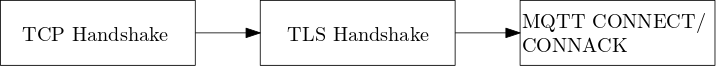
\includegraphics[scale=0.5]{tcp-tls-mqtt.png}\\
As such, using TLS increases the computation and network resources used when communicating. This is incongruent with MQTT's goal to be a lightweight protocol for low-power, low-resource devices, and adds complexity to the implementation of a properly secure MQTT software.\par
This report will focus on the implementation of TLS using digital certificates. There are 3 ways that certificate-based TLS is implemented in the case of an MQTT system:
\begin{enumerate}
	\item The broker has a certificate that is provided to clients that initialize the TLS handshake
	\begin{itemize}
		\item In this case, neither the broker nor the client authenticate each other
	\end{itemize}
	\item Clients keep a copy of trusted certificates, and check the certificate provided by the broker against their trusted certificates
	\begin{itemize}
		\item In this case, the client authenticates the broker
	\end{itemize}
	\item Clients pass a copy of their own certificate to the broker after verifying the broker's certificate, and the broker verifies that the client certificate has been signed by a trusted CA
	\begin{itemize}
		\item In this case, the broker and the client authenticate each other
	\end{itemize}
\end{enumerate}
As the TLS handshake occurs before the start of MQTT communication, troubleshooting MQTT over TLS is challenging. When an error occurs in the TLS handshake, it is almost always deemed fatal and by TLS protocol the broker and client must end their connection\cite{tls1.2errors}. Therefore, the broker and client are not able to engage in MQTT communications, requiring that errors be relayed between broker and client through the TLS header.

\section*{Experiment Setup}
broker 1 mosquitto version 1.6.9, Ubuntu 20.04.2 LTS 64-bit\\
broker 2 HiveMQ CE version 2020.2, Ubuntu 20.04.2 LTS 64-bit\\
client 1 mosquitto version 2.0.8, Windows Subsystem for Linux 4.4.0-19041-Microsoft 64-bit\\


\section*{Results}
\subsection*{Golang MQTT Packet Decoding}
Golang's \texttt{gopacket} library provides an API for capturing and decoding packets from a network interface. The \texttt{layers} library does not contain a layer for MQTT packets, so a collection of layers was created for each control packet type, as well as the MQTT fixed header.
\subsection*{Golang Packet Capture}
To accompany the MQTT layer decoders, a CLI packet capturing utility was built in Golang. 
\subsection*{MQTT over TLS using Certificates}

\begin{tabular}{  c l c | c c}
\hline
CA Certificate & Server Certificate & Client Certificate & Expected Result\\
\hline
valid & valid & valid & MQTT Communication
\end{tabular}
\section*{MQTT Software Defaults}
Mentioned in the MQTT specifications, an MQTT control packet's greatest possible size is 268, 435, 455 bytes (256 MiB less one byte). The only types of control packets that can achieve this length within the rules of the protocol are PUBLISH packets or SUBSCRIBE packets. The greatest possible payload for a MQTT 3.1.1 PUBLISH packet would be: 268, 435, 455 minus 1 byte for the packet type and flags, 4 bytes for the `Remaining Length', 2 bytes of the topic name length, and at minimum 1 byte of topic name, resulting in a payload of 256 MiB minus 9 bytes. The greatest possible payload for a MQTT 3.1.1 SUBSCRIBE packet would be: 268, 435, 455 minus 1 byte for packet type and flags, 4 bytes for the `Remaining Length', 2 bytes for the packet identifier, resulting in 256 MiB minus 8 bytes to be used to encode topic subscriptions. Each topic subscription requires 2 bytes for the topic name length, up to 65535 bytes for the topic name, and 1 byte for the desired QoS | allowing for at most 4095 maximum-size topic subscriptions. In the case of MQTT 5.0, these sizes are equal or lesser given that the variable header of each packet may contain bytes representing packet properties.\par
Given that MQTT is meant to be a lightweight protocol that uses few network resources, we would expect that MQTT clients and brokers will be sending control packets that are much smaller than the maximum packet size. Therefore, it would be reasonable that MQTT brokers enforce a smaller default maximum packet size to ensure that malicious actors cannot cause congestion by sending many large packets to the broker. 
\subsection*{mosquitto}

\subsection*{HiveMQ}
\section*{Future Work}
Retrieving TLS session keys from local MQTT traffic for debugging purposes?
\section*{Appendix A}
\begin{tabulary}{\textwidth}{cCc}
\hline
Option & Definition & Default Value\\
\hline
allow\_anonymous & Boolean value that determines whether clients that connect without providing a username are allowed to connect. If set to false then another means of connection should be created to control authenticated client access. & false\\
auth\_plugin\_deny\_special\_chars & If true then before an ACL check is made, the username/client id of the client needing the check is searched for the presence of either a '+' or '\#' character. If either of these characters is found in either the username or client id, then the ACL check is denied before it is sent to the plugin. & true\\

\end{tabulary}
\bibliographystyle{apalike}
\bibliography{comp4905}
\end{document}